\textbf{Chapter 10: QCD}

\textbf{Local Gauge Invariance in QED}

Local phase transformation of QED: U(1) trans. $\phi' = \phi e^{iq\chi(x)}$

To make QED invariant under that, must introduce photon field $A_\mu$ and modify Dirac eqn: $[i\gamma^\mu(\d_\mu + iqA_\mu) - m]\psi = 0$.

$A_\mu' = A_\mu - \d_\mu \chi(x)$

\textbf{Now for QCD}

Local phase transformation: SU(3) trans. $\phi' = \phi e^{ig\vec{\lambda} \cdot \vec{\theta}(x)}$

$\lambda_i$ = the Gell-Mann matrices

$\theta_i(x)$ = 8 spin-1 bosons (gluons)

Wavefunctions now include colour, $\psi = \psi_{\text{flav}}\chi_{\text{spin}}\xi_{\text{col}}\eta_{\text{spc}}$

\begin{align*}
    \lambda_1 &= \begin{bmatrix}
        0 & 1 & 0 \\
        1 & 0 & 0 \\
        0 & 0 & 0 \\
    \end{bmatrix}, \lambda_2 = \begin{bmatrix}
        0 & -i & 0 \\
        i & 0 & 0 \\
        0 & 0 & 0 \\
    \end{bmatrix}\\
    \lambda_3 &= \begin{bmatrix}
        1 & 0 & 0 \\
        0 & -1 & 0 \\
        0 & 0 & 0 \\
    \end{bmatrix}, \lambda_4 = \begin{bmatrix}
        0 & 0 & 1 \\
        0 & 0 & 0 \\
        1 & 0 & 0 \\
    \end{bmatrix} \\
    \lambda_5 &= \begin{bmatrix}
        0 & 0 & -i \\
        0 & 0 & 0 \\
        i & 0 & 0 \\
    \end{bmatrix}, \lambda_6 = \begin{bmatrix}
        0 & 0 & 0 \\
        0 & 0 & 1 \\
        0 & 1 & 0 \\
    \end{bmatrix} \\
    \lambda_7 &= \begin{bmatrix}
        0 & 0 & 0 \\
        0 & 0 & -i \\
        0 & i & 0 \\
    \end{bmatrix}, \lambda_8 = \frac{1}{\sqrt{3}}\begin{bmatrix}
        1 & 0 & 0 \\
        0 & 1 & 0 \\
        0 & 0 & -2 \\
    \end{bmatrix} \\
\end{align*}

\textbf{QCD Feynman Rules}

Quarks: same as QED leptons

Gluons: same as QED photons

Gluon prop: $-\frac{ig_{\mu\nu}}{q^2}\delta^{ab}$

Vertices (qqg): $-ig_s\frac{1}{2}\lambda^a_{ji}\gamma^\mu$, i, j = (1,2,3) = (r, g, b) for initial, final quark colours

Other vertex terms exist but won't be tested.

Remember to have colour-neutral initial / final states

\textbf{Colour factors} $C(ik \to jl) = \frac{1}{4}\sum_{a=1}^8 \lambda^{a}_{ji}\lambda^a_{lk}$ (r=1, g=2, b=3). Remember colour conservation when applicable!

At each vertex, put the adjoint first, e.g. $u_i \to g+u_j$ gives $\lambda^a_{ji}$.

\begin{center}
    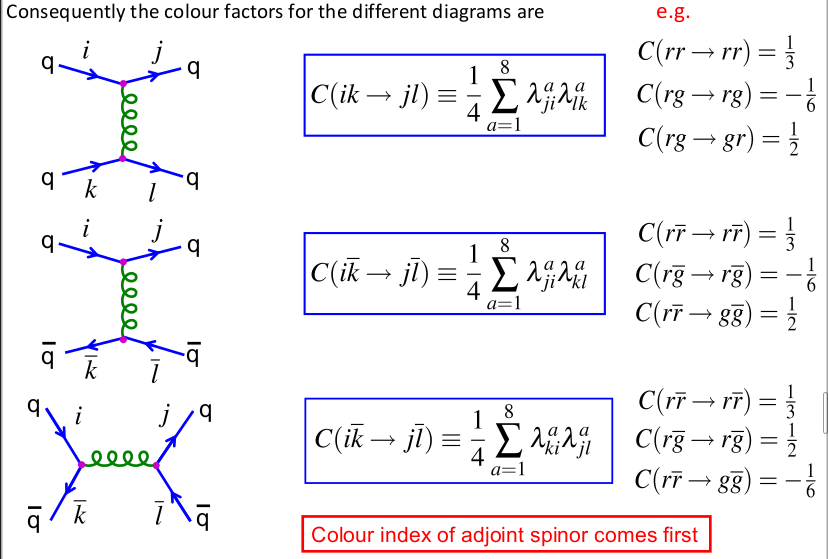
\includegraphics[width=\linewidth]{images/colour_factors.png}
\end{center}

\begin{align*}
    \expval{|C|^2} &= \frac{1}{9}\sum_{ijkl=1}^3 |C(ij\to kl)|^2 \\
\end{align*}

$M_{QCD} = C M_{QED}$ for our purposes, also replace $e \to g_s^2$.

At low energies can't do QCD since $a_s \approx 1$, but at high energies can use perturbation theory just like QED = ``asymptotic freedom.''
